\documentclass{article}
\usepackage[utf8]{inputenc}
\usepackage{graphicx}
\usepackage{wrapfig}
\usepackage{array}
\usepackage{siunitx}
\usepackage{xcolor}
\usepackage{multicol}
\usepackage{amssymb}
\setlength{\columnseprule}{1pt}

\title{Experiment Based on Network Theorems (KCL,KVL) \\ Lab Report 2 \\ ELP100}
\author{Yash Agarwal \\ 2021EE10638 \\ Group 29}
\date{April 15, 2022}

\begin{document}
\pagecolor{yellow!15}
\maketitle
\vspace{20px}
\tableofcontents
\newcolumntype{V}{>{\centering\arraybackslash} m{.4\linewidth} }
\newpage
\section{Kirchhoff's Laws}
\vfill
\subsection{Aim}
To verify the Kirchhoff's Current Law(KCL) and Kirchhoff's Voltage Law(KVL) in a circuit.
\vfill
\subsection{Apparatus}
\begin{enumerate}
    \item Multiple Power Supply
    \item Resistors (1 of 47 $\Omega$, 1 of 470 $\Omega$, 2 of 100 $\Omega$, 2 of 220 $\Omega$ and 1 of 150 $\Omega$)
    \item Multimeter
    \item Connecting Wires
    \item Breadboard
\end{enumerate}
\vfill
\subsection{Theory}
\vfill
\subsubsection{Kirchhoff's Current Law}

\begin{wrapfigure}{R}{0.3\textwidth}
\fcolorbox{black}{white}{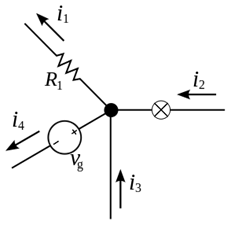
\includegraphics[width=0.25\textwidth]{Picture2.png}}
\end{wrapfigure}

The sum of currents coming into any node (junction) in an electrical circuit is equal to the total of currents flowing out of that node, or the algebraic sum of currents in a network of conductors meeting at a point is zero.
The conservation of charge is the foundation of this law. For example, at the darkest point, the net current is zero, implying that:
\[i_1+i_4=i_2+i_3\]

\vfill
\subsubsection{Kirchhoff's Voltage Law}

\begin{wrapfigure}{R}{0.3\textwidth}
\fcolorbox{black}{white}{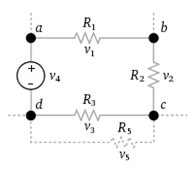
\includegraphics[width=0.25\textwidth]{Picture1.png}}
\end{wrapfigure}

The directed sum of the electrical potential difference (voltage) around any closed network is zero, or, to put it another way, the algebraic sum of the product of conductor resistances and currents in a closed loop equals the total emf available in that loop. The sum of all the voltages surrounding a loop, is zero, as shown by this equation:
\[V_1+V_2+V_3-V_4 = 0 \]

\newpage
\subsection{Circuit Setup}
\vspace{5px}
\subsubsection{Circuit}
\begin{center}
    \fcolorbox{black}{white}{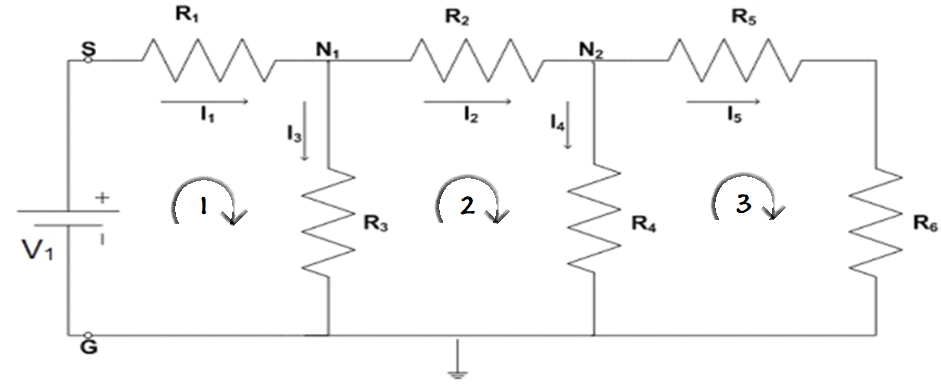
\includegraphics[width=0.75\textwidth]{Picture3.png}}
\end{center}

$Here, V_1 = 5V,\ R_1 = R_2 = 100 \Omega, \ R_3 = R_4 = 220 \Omega,\ R_5 = 47 \Omega,\ R_6 = 150 \Omega$
\subsubsection{Breadboard}


\begin{multicols}{2}
\begin{center}
\fcolorbox{black}{white}{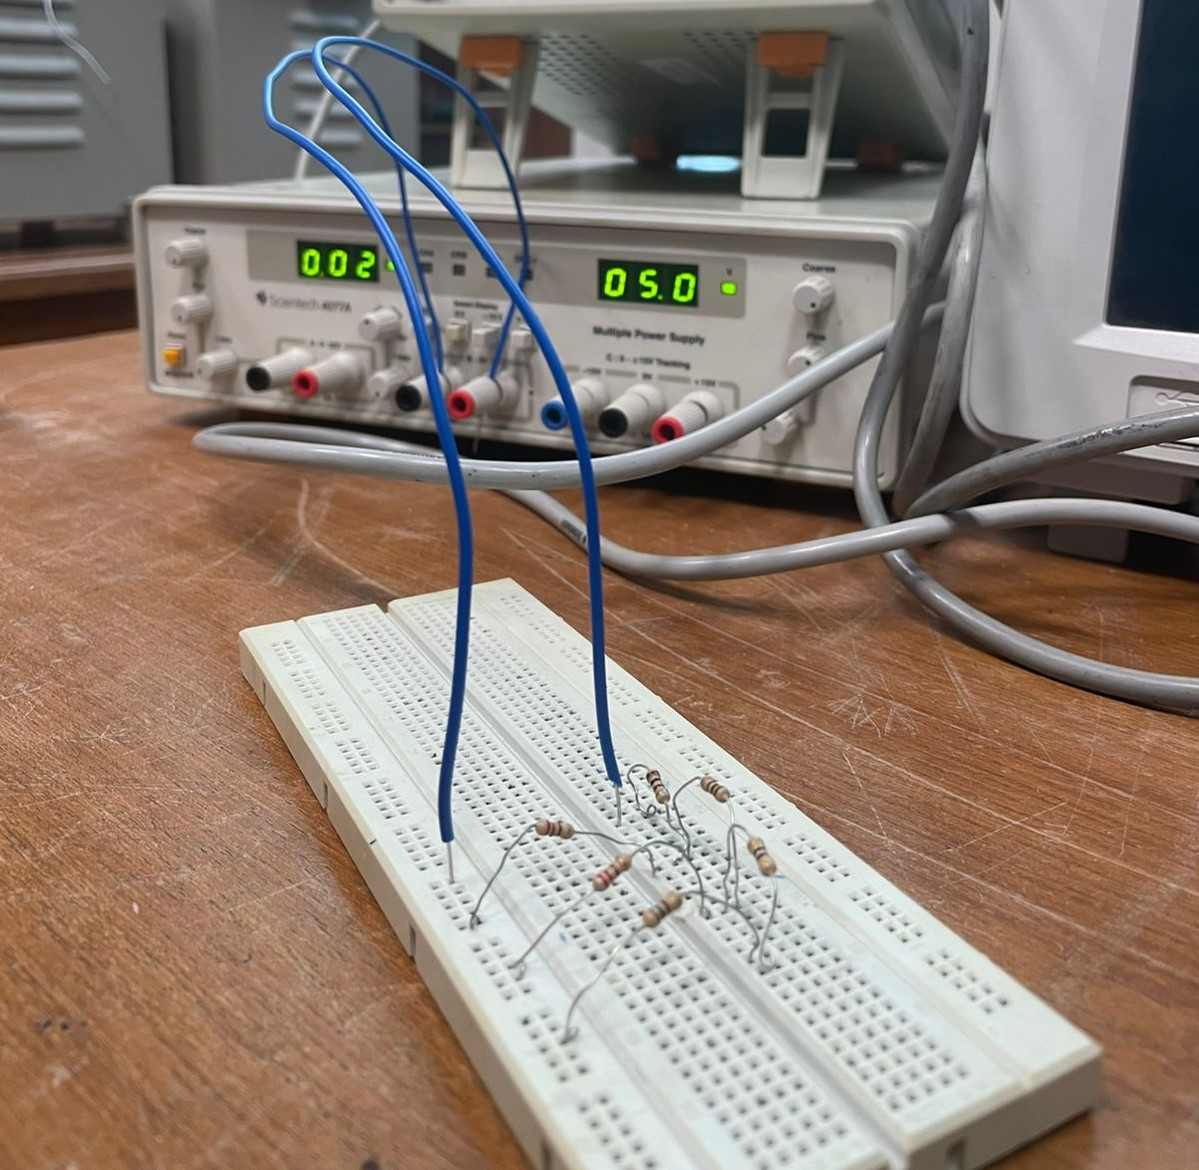
\includegraphics[width=0.9\columnwidth, height=150px]{Breadboard 1.jpeg}} \\ \vspace{5px}
Breadboard without 470 $\Omega$ Resistor \\

\columnbreak

\fcolorbox{black}{white}{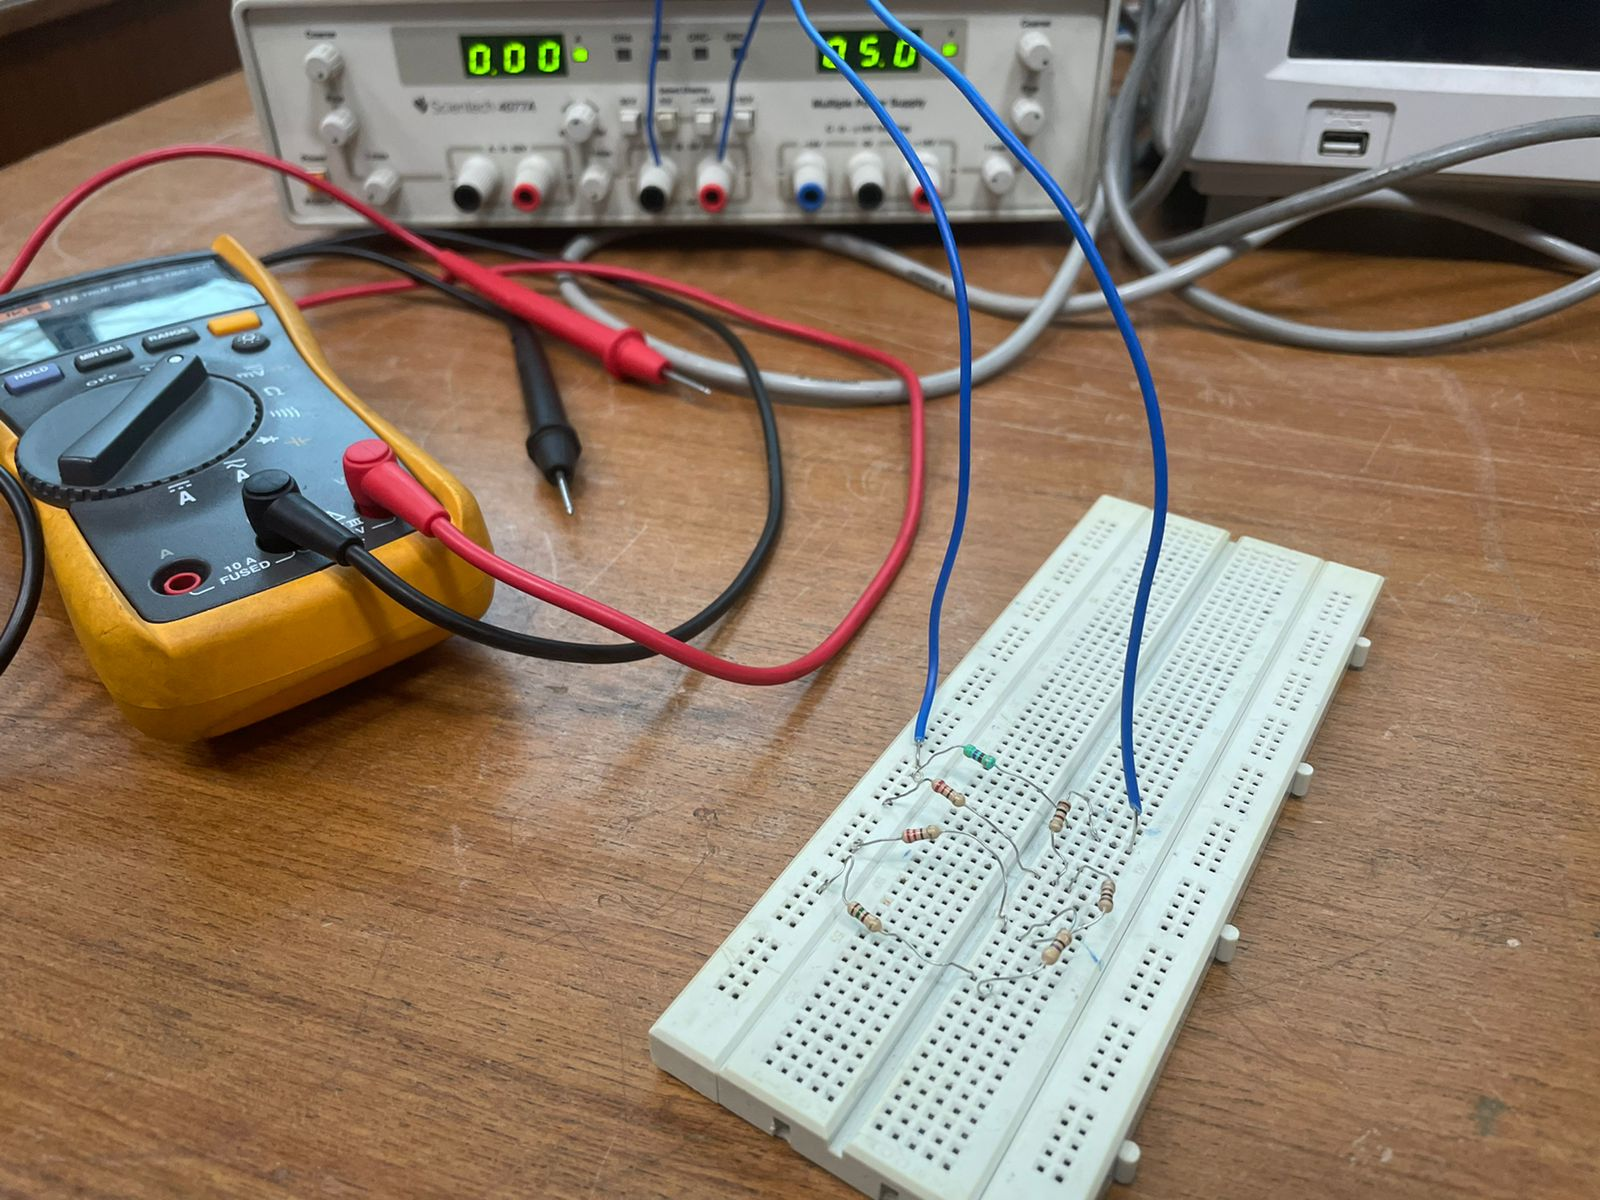
\includegraphics[width=0.9\columnwidth, height=150px]{Breadboard 2.jpeg}} \\ \vspace{5px}
Breadboard with 470 $\Omega$ Resistor
\end{center}
\end{multicols}


\subsection{Observation}
\vspace{5px}
\begin{center}
\begin{tabular}{|c | c | c |} 
 \hline
    \ & \ & \ \\
    Resistors & Measured Voltage (V) & Calculated Current (mA) \\ [1em]
    \hline
    \ & \ & \ \\
    $R_1(100 \Omega$) & $V_{R_1}=$ \ 2.47V & $i_1=$ \ 24.7mA  \\
    $R_2(100 \Omega$) & $V_{R_2}=$ \ 1.27V & $i_2=$ \ 12.7mA  \\
    $R_3(220 \Omega$) & $V_{R_3}=$ \ 2.58V & $i_3=$ \ 11.7mA  \\
    $R_4(220 \Omega$) & $V_{R_4}=$ \ 1.31V & $i_4=$ \ 5.95mA  \\
    $R_5(047 \Omega$) & $V_{R_5}=$ \ 0.31V & $i_5=$ \ 6.59mA  \\
    $R_6(150 \Omega$) & $V_{R_6}=$ \ 1.00V & $i_6=$ \ 6.66mA  \\
    \ & \ & \ \\
 \hline
\end{tabular}
\end{center}

\newpage

\subsection{Verification of Kirchhoff's Current Law}
\vspace{5px}
\subsubsection{Node 1}
Incoming Current: $i_1=$ \ 24.7mA \\
Outgoing Current: $i_2 + i_3=$ \ 12.7mA + 11.7mA = 24.4mA $\approx$ Incoming Current. \\
\noindent
As Incoming Current is approximately equal to Outgoing Current, Kirchhoff's Current Law is verified.

\subsubsection{Node 2}
Note: $i_5=i_6$, thus we take $i_5$ as the average of obtained values of $i_5$ and $i_6$. Thus, $i_5=i_6= \ 6.63mA$ \\

\noindent
Incoming Current: $i_2=$ \ 12.7mA \\
Outgoing Current: $i_4 + i_5=$ \ 5.95mA + 6.63mA = 12.58mA $\approx$ Incoming Current. \\ 
\noindent
As Incoming Current is approximately equal to Outgoing Current, Kirchhoff's Current Law is verified.

\subsection{Verification of Kirchhoff's Current Law}
\vspace{5px}
\subsubsection{Loop 1}
Potential Drop: $V_1-V_{R_1}-V_{R_3}=$ \ 5V - 2.47V - 2.58V = -0.05V $\approx$ 0V

\noindent
As Potential Drop is approximately equal to 0, Kirchhoff's Voltage Law is verified.

\subsubsection{Loop 2}
Potential Drop: $V_{R_3}-V_{R_2}-V_{R_4}=$ \ 2.58V - 1.27V - 1.31V = 0V $\approx$ 0V

\noindent
As Potential Drop is approximately equal to 0, Kirchhoff's Voltage Law is verified.

\subsubsection{Loop 3}
Potential Drop: $V_{R_4}-V_{R_5}-V_{R_6}=$ \ 1.31V - 1V - 0.31V = 0V $\approx$ 0V

\noindent
As Potential Drop is approximately equal to 0, Kirchhoff's Voltage Law is verified.
\subsection{Change in $i_5$ when $R_7=470\Omega$ is connected across SG}
$V'_5=$ \ 0.309V, \  $\therefore$ $i'_5=$ \  6.57mA. Thus, there is negligible change in $i_5$. The variation in the reading may be due to some finite resistance in the connecting wires.

\subsection{Conclusion}
Hence, we were able to verify the Kirchhoff’s Circuit Laws for a given circuit.
\newpage

\section{Verification of Superposition Principle}
\subsection{Aim}
To verify the Superposition Principle 

\subsection{Apparatus}
\begin{enumerate}
    \item Multiple Power Supply ( 2 Needed )
    \item Resistors (1 of 47 $\Omega$, 1 of 470 $\Omega$, 2 of 100 $\Omega$, 2 of 220 $\Omega$ and 1 of 150 $\Omega$)
    \item Multimeter
    \item Connecting Wires
    \item Breadboard
\end{enumerate}

\subsection{Theory}

The superposition theorem for electrical circuits states that for any branch of a bilateral linear circuit with more than one independent source, the response (voltage or current) in any branch equals the algebraic sum of the responses caused by each independent source acting alone, where all other independent sources are replaced by their internal resistance. This theorem's steps are as follows:
\begin{itemize}
\item Using a short circuit to replace all other independent voltage sources (eliminating potential differences, i.e. V=0).
\item Using an open circuit to replace all other independent current sources (thus removing current, i.e. i=0).
\end{itemize}
\begin{center}
\fcolorbox{black}{white}{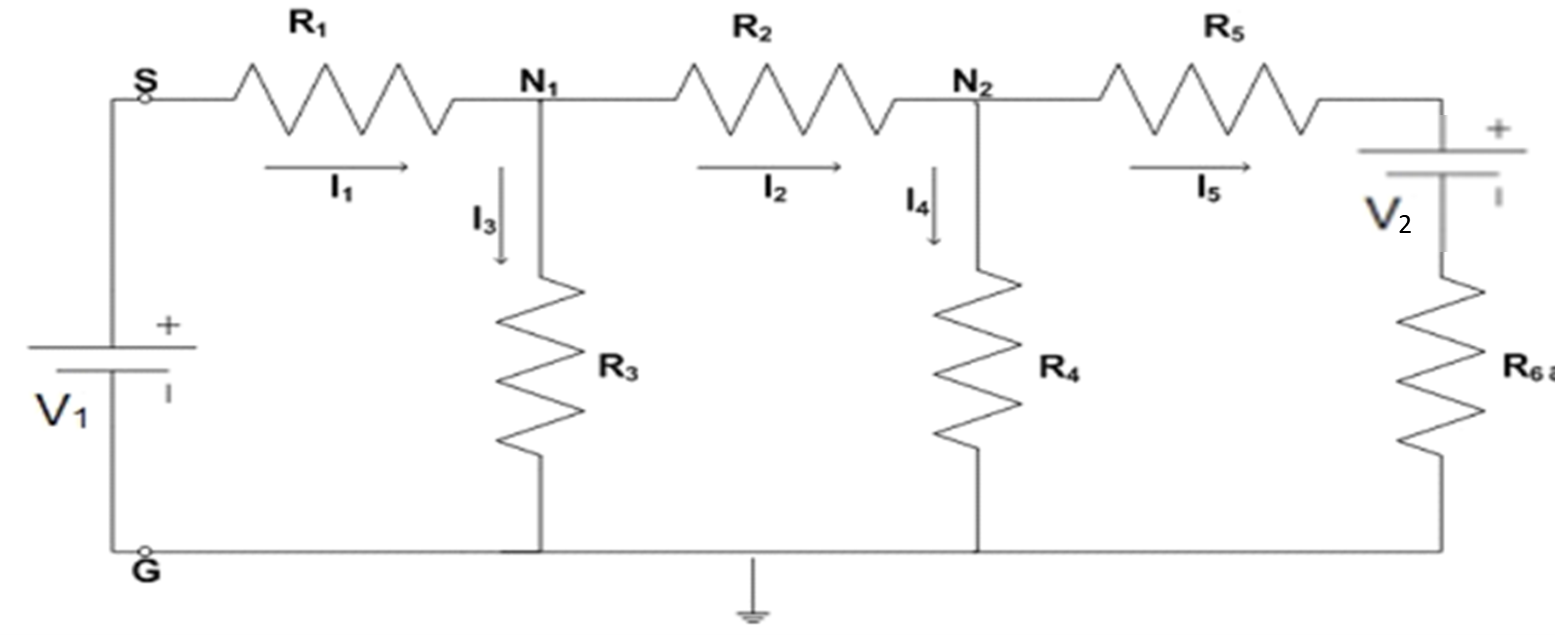
\includegraphics[width=0.8\textwidth]{Picture4.png}}
\end{center}

For example, in a circuit with two voltage sources, the current flowing through a resistor is because of both of them. When each of the sources is short-circuited, current through the resistor is $i_1$ and $i_2$. Then, using the principle of superposition,
\[ i_1 + i_2 = i \]

\newpage

\subsection{Setup}
The setup remains the same as the setup in Part 1 but now another voltage source $V_2$ is applied in series with $R_5$. Then $i_2$ is obtained, and it is also done when only $V_2$ is applied, i.e. when $V_1$ is shorted.

\subsection{Breadboard}
\begin{multicols}{2}
\begin{center}
\fcolorbox{black}{white}{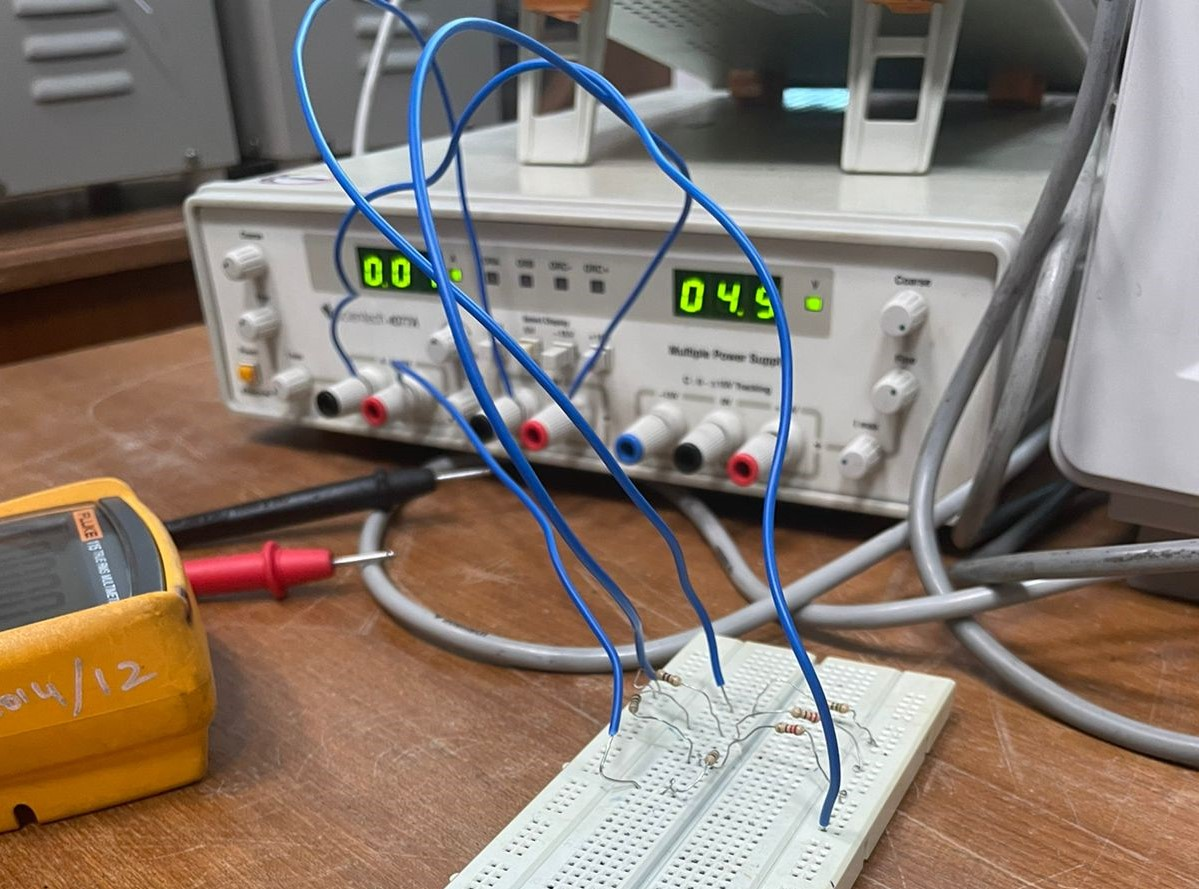
\includegraphics[width=0.9\columnwidth, height=150px]{Breadboard 3.jpeg}} \\ \vspace{5px}
Breadboard with both $V_1$ and $V_2$ \\

\columnbreak

\fcolorbox{black}{white}{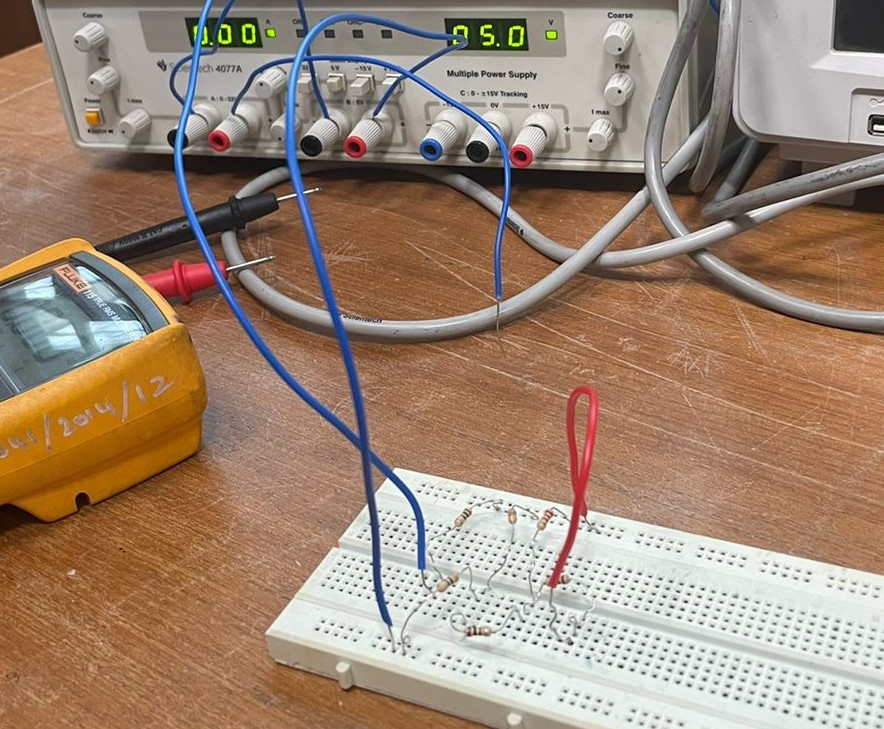
\includegraphics[width=0.9\columnwidth, height=150px]{Breadboard 4.jpeg}} \\ \vspace{5px}
Breadboard with $V_1$ shorted
\end{center}
\end{multicols}
\subsection{Observation}
\begin{center}
\begin{tabular}{| c | c | c |} 
 \hline
    \ & \ & \ \\
    Conditions & $V_{R_2}$ & $i_2$ \\
    \ & \ & \ \\
    \hline
    \ & \ & \ \\
    Only $V_1$ & 1.27V & 12.7mA \\
    Only $V_2$ & -0.976V & -9.76mA \\
    Both $V_1 \ and \ V_2$ & 0.277V & 2.77mA \\
    \ & \ & \ \\
    \hline
\end{tabular}
\end{center}
\subsection{Calculation}
$i_2$ when only $V_1$ is connected: 12.7mA \\
$i_2$ when only $V_2$ is connected: -9.76mA \\

\noindent
Thus, $i_2$ when both $V_1 \ and \ V_2$ are connected is: 12.7mA - 9.76mA =  2.94mA $\approx$ 2.77mA.


\subsection{Conclusion}
Hence, we have verified the Superposition Theorem.

\newpage







\section{Wheatstone Bridge}
\subsection{Aim}
To measure input resistance and study the effect on voltage and current on some modifications in Wheatstone Bridge.

\subsection{Apparatus}
\begin{enumerate}
    \item Multiple Power Supply
    \item Resistors (5 of 120 $\Omega$)
    \item Multimeter
    \item Connecting Wires
    \item Breadboard
\end{enumerate}

\subsection{Theory}

\begin{wrapfigure}{R}{0.3\textwidth}
    \fcolorbox{black}{white}{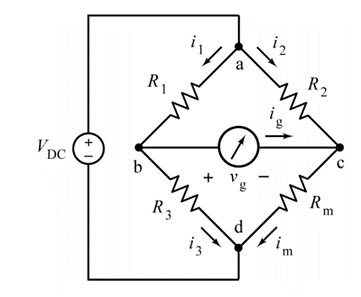
\includegraphics[width=0.3\textwidth]{Picture5.png}}
\end{wrapfigure}

Wheatstone bridge is a type of an electrical circuit which is used to measure an unknown resistance by balancing two legs. The galvanometer is used to detect the condition $i_g = 0$ . When the circuit satisfies the mentioned condition, we say that “the bridge is balanced”.

Because the galvanometer is a type of ammeter, $v_g = 0$ . (It’s always true that $v_g=0$ , whether the bridge is balanced or not. When the bridge is balanced it is also true that $i_g=0$ .)

The condition of balanced bridge is that:
\[ \frac{R_1}{R_3}=\frac{R_2}{R_m} \; or \; R_m= \frac{R_2 \times R_3}{R_1}\]

\subsection{Setup}
\begin{center}
    \fcolorbox{black}{yellow!15}{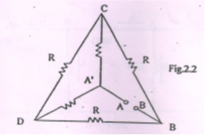
\includegraphics[width=0.5\textwidth]{Picture6.png}} \\
    \vspace{5px}
    Where $R=120 \Omega$
\end{center}

\newpage

\subsection{Breadboard}
\begin{center}
    \fcolorbox{black}{white}{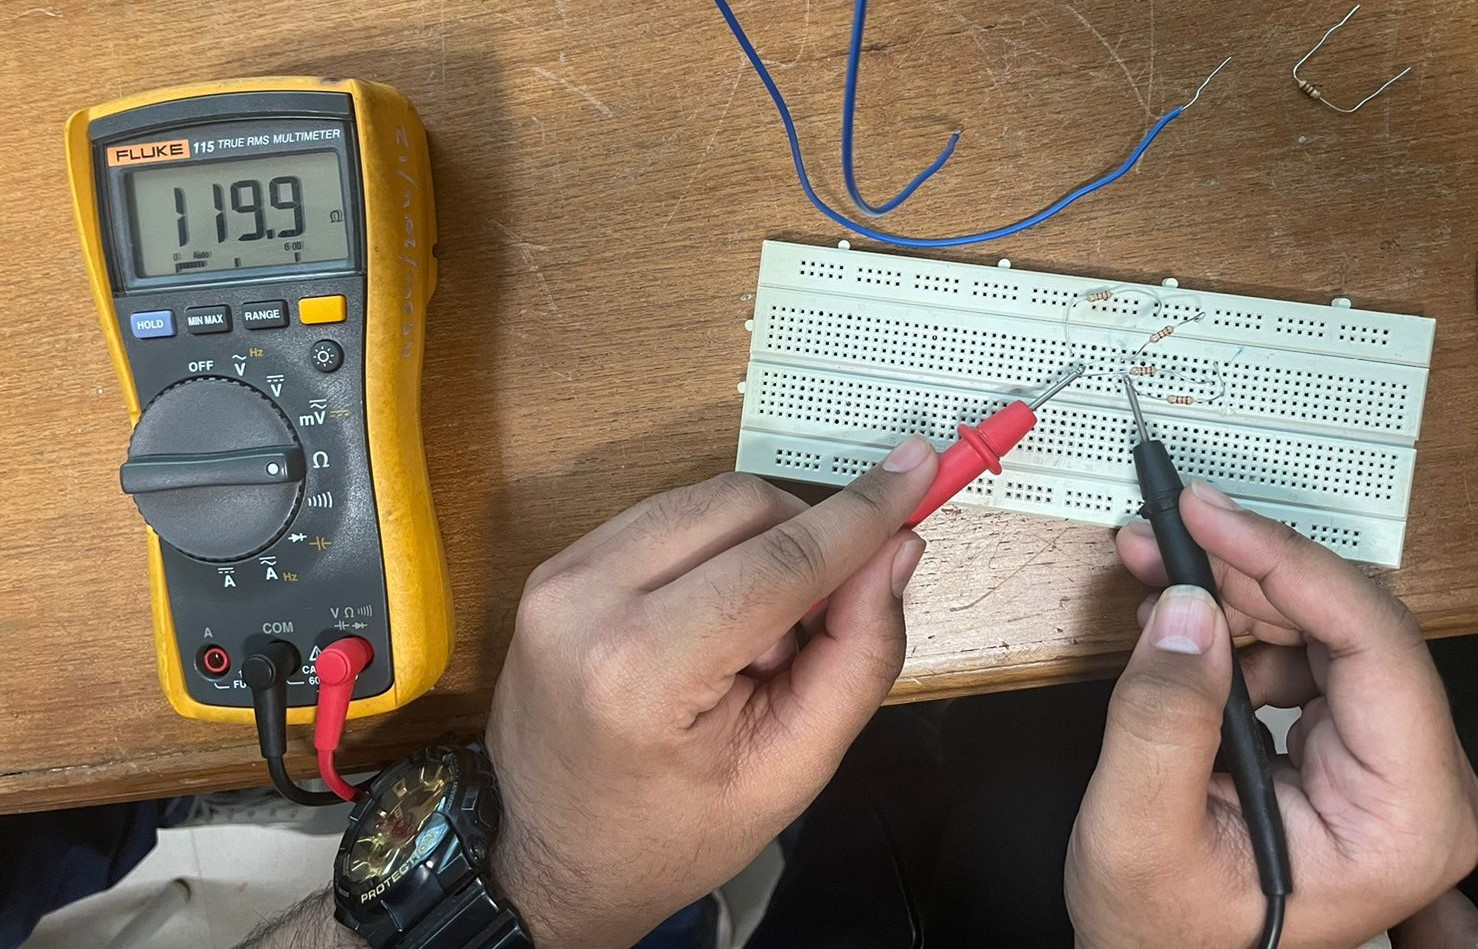
\includegraphics[width=0.75\textwidth]{Breadboard 5.jpeg}} \\
    \vspace{5px}
    Measuring input resistance between AB
\end{center}

\subsection{Observation}
\begin{itemize}
    \item Measured resistance between AB: $119.9 \Omega$
    \item Measured Voltage $V_{BC}:$ 2.46V
    \item Measured Voltage $V_{BD}:$ 2.44V
    \item Measured Voltage $V_{CD}:$ 0.02V
    \item CD Short Circuited: $R=120.1 \Omega$, \  i=0.042A
    \item CD Open: $R=120.2 \Omega$, \ i=0.042A
\end{itemize}


As $\frac{R_1}{R_2}=\frac{R_3}{R_4}$ (All Resistance's are $120 \Omega$), $V_{CD}$ should be 0 as the Wheatstone bridge is balanced. But since practically the value of resistances may vary a bit in real life, $V_{CD}$ is not exactly 0 but approximately 0. Also $V_{BC}$ and $V_{BD}$ should be equal. But there is slight deviation. But, they follow KVL as $V_{BC}-V_{CD}-V_{BD}=0$.

As it is a balanced Wheatstone bridge, it doesnt matter whether we short or keep open or put any resistance across CD. There is small deviation in values which might be due to internal resistance, resistance of wires, etc, which we didnt account for.

\subsection{Conclusion}
Hence we were able to verify the concepts of Wheatstone Bridge and observed that it doesnt matter if we put a resistance across CD, short it, or keep it open.

\newpage

\section{Sources of Error}
\begin{itemize}
    \item Loose connections.
    \item Resistance in wires and change due to temperature.
    \item Connections changed while circuit is powered.
\end{itemize}

\vspace{15px}

\section{Precautions}

\begin{itemize}
    \item Insulated tools should be used.
    \item Electric wires should be properly snipped.
    \item Proper shoes should be worn.
    \item Circuit should not be left powered for long time.

\end{itemize}

\vspace{15px}

\section{Concluding Remarks}
We used this experiment to test the electrical circuit ideas and laws that we had previously learned about. In an electric circuit, we confirmed Kirchhoff's Voltage and Current law. We can also see that any resistance placed in parallel to the voltage source has no effect on the currents in the circuit. We also proved that linear electrical circuits have superposition theorem. We used voltage sources and shorted other sources to demonstrate the validity of the superposition theorem experimentally (within experimental error). We also tested the Wheatstone bridge circuit, determining the resistance and voltage by making several alterations, such as short-circuiting and open-circuiting the middle leg, to demonstrate the independence of a balanced Wheatstone Bridge.
\end{document}
